
\section{Modelos de lenguaje y generación de lenguaje}
\begin{itemize}
\item La modelización del lenguaje es la tarea de asignar una probabilidad a las oraciones en un lenguaje.
\item Por ejemplo, ¿cuál es la probabilidad de ver la oración "el perro perezoso ladró ruidosamente"?
\item La tarea se puede formular como la tarea de predecir la probabilidad de ver una palabra condicionada a las palabras anteriores:
\begin{displaymath}
P(w_i | w_1, w_2, \cdots, w_{i-1}) = \frac{P(w_1, w_2, \cdots, w_{i-1}, w_i)}{P(w_1, w_2, \cdots, w_{i-1})}
\end{displaymath}
\item Las RNN se pueden utilizar para entrenar modelos de lenguaje vinculando la salida en el tiempo $i$ con su entrada en el tiempo $i + 1$.
\item Esta red se puede utilizar para generar secuencias de palabras o frases aleatorias.
\item Proceso de generación: predecir una distribución de probabilidad sobre la primera palabra condicionada al símbolo de inicio y seleccionar una palabra aleatoria de acuerdo con la distribución predicha.
\item Luego, predecir una distribución de probabilidad sobre la segunda palabra condicionada a la primera, y así sucesivamente, hasta predecir el símbolo de fin de secuencia $</$s$>$.
\item Después de predecir una distribución sobre los siguientes símbolos de salida $P(t_i = k | t_{1:i-1})$, se elige un token $t_i$ y su vector de incrustación correspondiente se alimenta como entrada al siguiente paso.
         \begin{figure}[h]
        	\centering
        	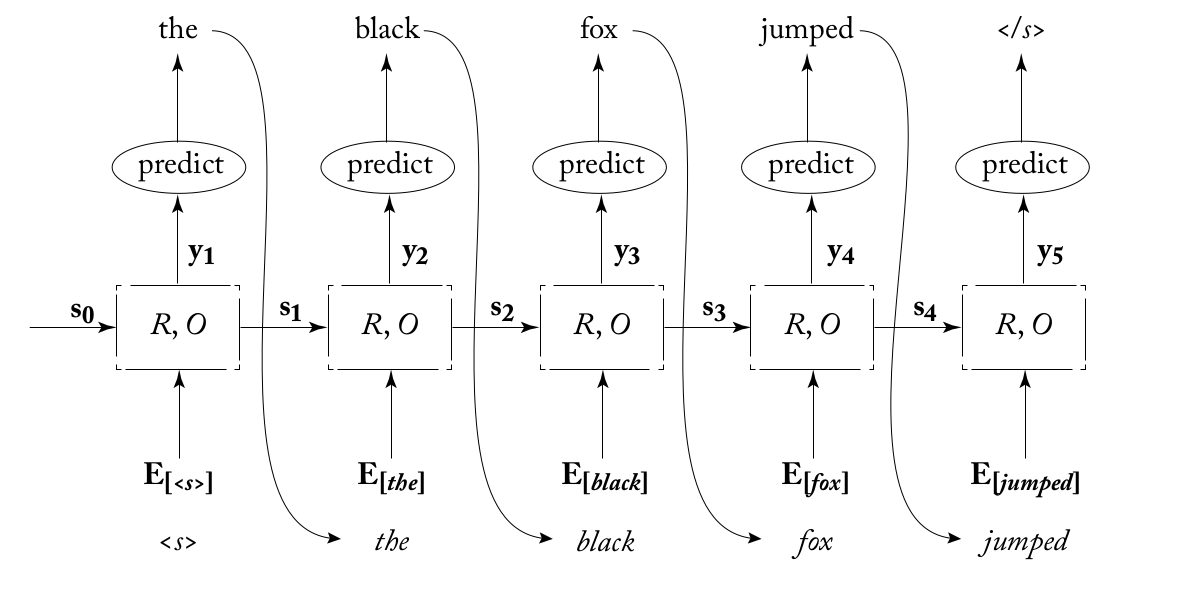
\includegraphics[scale = 0.25]{pics/generator.png}
        	\caption{Arquitectura de generación de lenguaje con una RNN.}
        \end{figure}
\item Teacher-forcing: durante el \textbf{entrenamiento}, se alimenta al generador con la palabra anterior verdadera, incluso si su propia predicción le asignó una pequeña probabilidad.
\item Es probable que el generador haya generado una palabra diferente en este estado durante la \textbf{prueba}.
\end{itemize}





\section{Problemas de secuencia a secuencia}
Casi cualquier tarea en NLP se puede formular como un problema de secuencia a secuencia (o generación condicionada), es decir, generar secuencias de salida a partir de secuencias de entrada. Las secuencias de entrada y salida pueden tener longitudes diferentes.
\begin{itemize}
\item Traducción automática: de un idioma fuente a un idioma objetivo.
\item Resumen: de texto largo a texto corto.
\item Diálogo (chatbots): de las intervenciones anteriores a la siguiente intervención.
\end{itemize}

\subsection{Generación condicionada}
\begin{itemize}
\item Si bien utilizar la RNN como generador es un ejercicio interesante para demostrar su fortaleza, el verdadero poder del generador de RNN se revela cuando se pasa a una generación condicionada o un marco de codificador-decodificador.
\item Idea central: usar dos RNN.
\item Codificador: se utiliza una RNN para codificar la entrada fuente en un vector $\overrightarrow{c}$.
\item Decodificador: se utiliza otra RNN para decodificar la salida del codificador y generar la salida objetivo.
\item En cada etapa del proceso de generación, el vector de contexto $\overrightarrow{c}$ se concatena a la entrada $\hat{t}_j$ y la concatenación se alimenta a la RNN.
\begin{frame}{Marco codificador-decodificador}
         \begin{figure}[h]
        	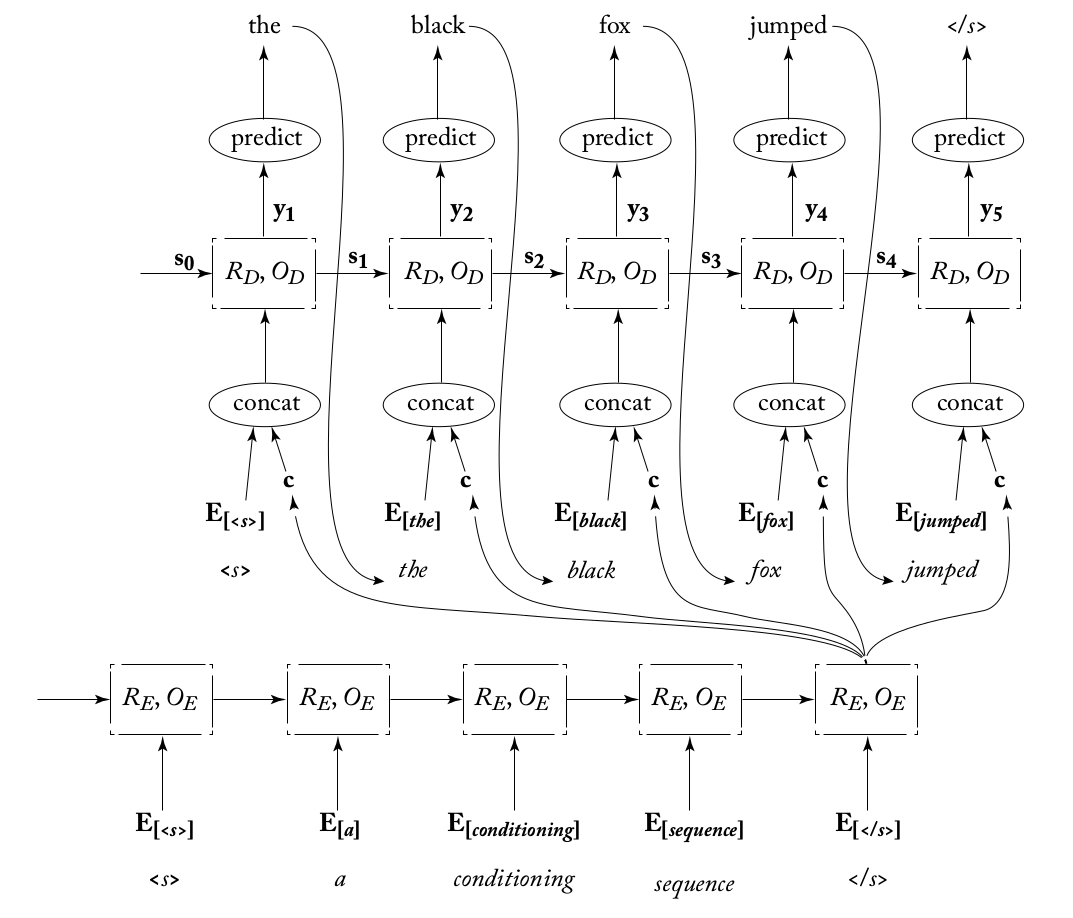
\includegraphics[scale = 0.32]{pics/seqseq.png}
        \end{figure}
\end{frame}
\item Esta configuración es útil para mapear secuencias de longitud $n$ a secuencias de longitud $m$.
\item El codificador resume la oración fuente en un vector $\vec{c}$.
\item Luego, la RNN del decodificador se utiliza para predecir (utilizando un objetivo de modelado del lenguaje) las palabras de la secuencia objetivo condicionadas tanto a las palabras predichas anteriormente como a la oración codificada $\vec{c}$.
\item Las RNN del codificador y del decodificador se entrenan conjuntamente.
\item La supervisión solo ocurre para la RNN del decodificador, pero los gradientes se propagan hasta la RNN del codificador.
\end{itemize}


\paragraph{Gráfico de entrenamiento de secuencia a secuencia}
         \begin{figure}[h]
        	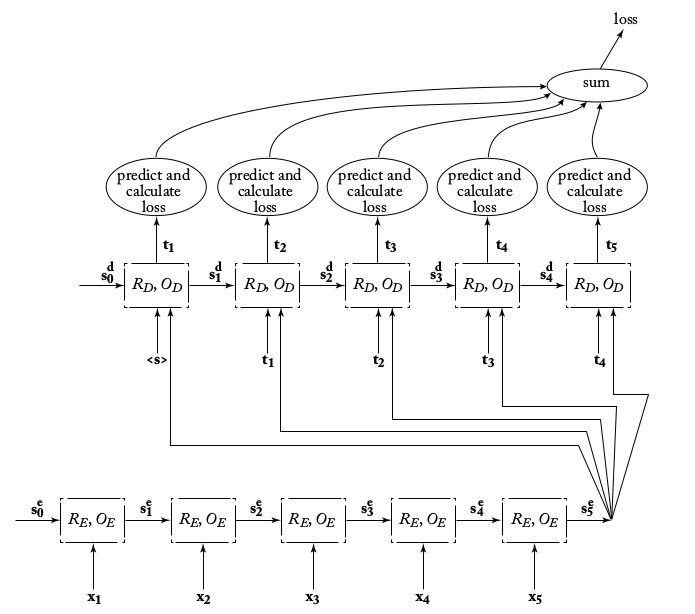
\includegraphics[scale = 0.35]{pics/seq2se2train.png}
        \end{figure}





\paragraph{Traducción automática neuronal}
         \begin{figure}[h]
        	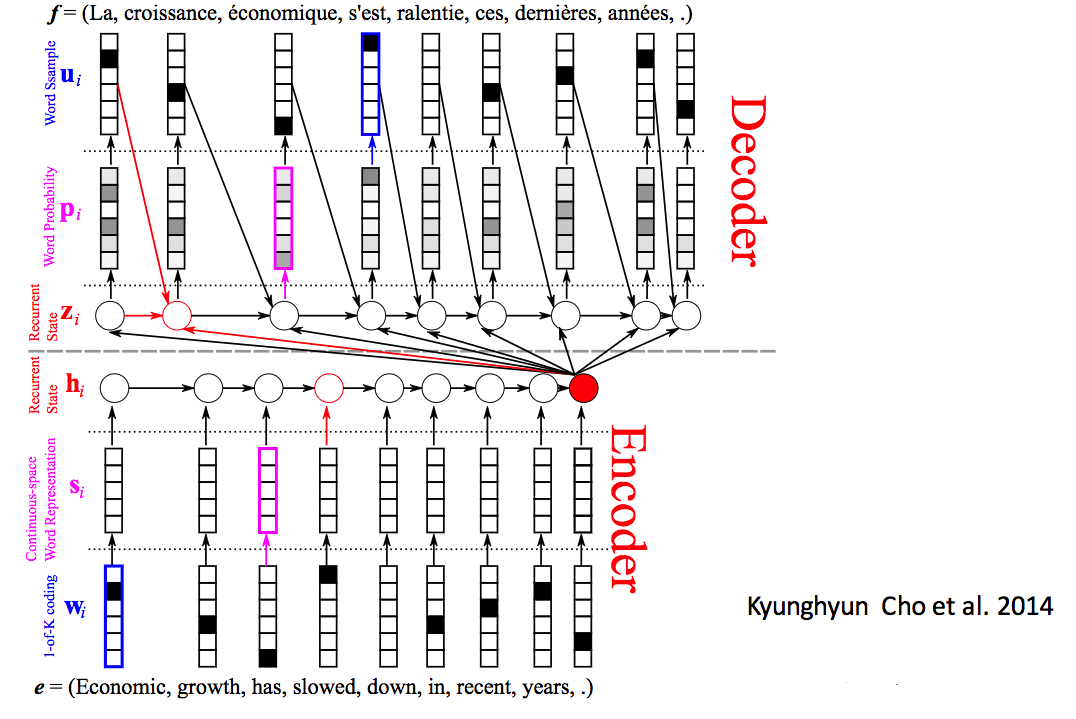
\includegraphics[scale = 0.25]{pics/mt.png}
        \end{figure}

\paragraph{Progreso de BLEU en traducción automática}
         \begin{figure}[h]
        	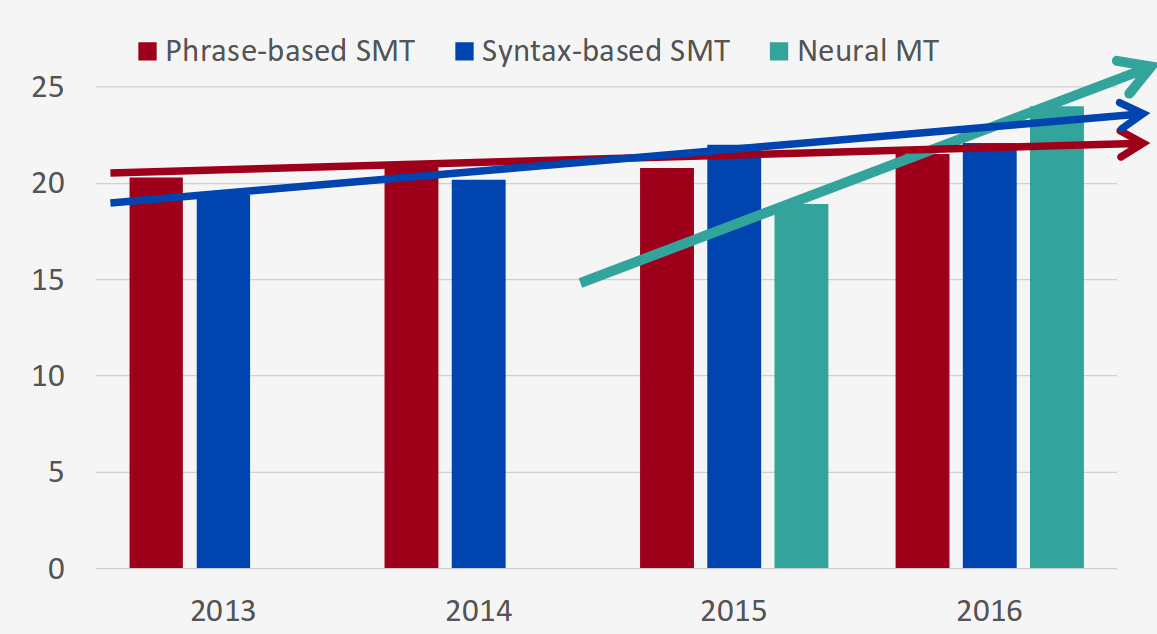
\includegraphics[scale = 0.35]{pics/nmt_progress.png}
        \end{figure}
[Edinburgh En-De WMT]
\footnotetext{fuente: \url{http://www.meta-net.eu/events/meta-forum-2016/slides/09_sennrich.pdf}}


\section{Enfoques de decodificación}
\begin{itemize}
\item El decodificador tiene como objetivo generar la secuencia de salida con la puntuación máxima (o probabilidad máxima), es decir, de modo que se maximice $\sum_{i=1}^{n}P(\hat{t}_i | \hat{t}_{1:i-1})$.
\item La naturaleza no markoviana de la RNN significa que la función de probabilidad no se puede descomponer en factores que permitan una búsqueda exacta utilizando la programación dinámica estándar.
\item Búsqueda exacta: encontrar la secuencia óptima requiere evaluar todas las secuencias posibles (computacionalmente prohibitivo).
\item Por lo tanto, solo tiene sentido resolver aproximadamente el problema de optimización anterior.
\item Búsqueda por greedy: elegir la predicción (palabra) de mayor puntuación en cada paso.
\item Esto puede dar como resultado una probabilidad global subóptima y llevar a prefijos seguidos de eventos de baja probabilidad.
\end{itemize}


\begin{figure}[h]
  \centering
  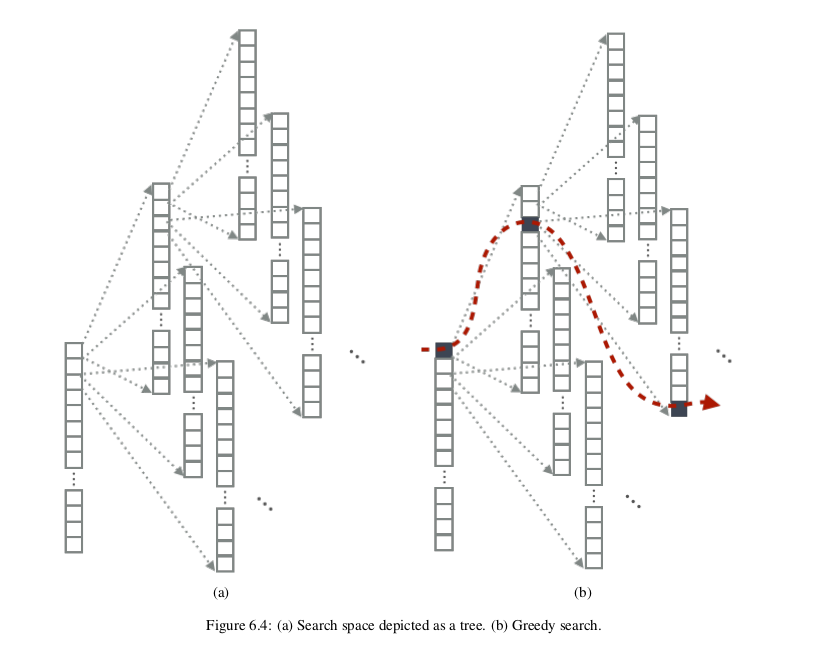
\includegraphics[scale=0.3]{pics/greedysearch.png}
  \caption{Búsqueda greedy en la decodificación de secuencia a secuencia.}
\end{figure}



\subsection{Búsqueda Beam}
\begin{itemize}
\item La búsqueda Beam interpolan entre la búsqueda exacta y la búsqueda greedy al cambiar el tamaño $K$ de las hipótesis mantenidas durante todo el procedimiento de búsqueda \cite{cho2015natural}.
\item El algoritmo de búsqueda Beam funciona en etapas.
\item Primero se eligen las $K$ palabras de inicio con la probabilidad más alta.
\item En cada paso, cada secuencia candidata se expande con todas las posibles siguientes etapas.
\item Cada paso candidato se puntúa.
\item Se conservan las $K$ secuencias con las probabilidades más probables y se eliminan todas las demás candidatas.
\item El proceso de búsqueda puede detenerse para cada candidato por separado ya sea alcanzando una longitud máxima, alcanzando un token de fin de secuencia o alcanzando una probabilidad umbral.
\item Se selecciona la oración con la probabilidad global más alta.
\end{itemize}

\footnotetext{Más información en: \url{https://machinelearningmastery.com/beam-search-decoder-natural-language-processing/}}

\section{Generación condicionada con atención}
\begin{itemize}
\item En las redes codificador-decodificador, la oración de entrada se codifica en un solo vector, que luego se utiliza como contexto de condicionamiento para un generador RNN.
\item Esta arquitectura obliga al vector codificado $\vec{c}$ a contener toda la información requerida para la generación.
\item ¡No funciona bien para oraciones largas!
\item También requiere que el generador pueda extraer esta información del vector de longitud fija.
\item "¡No puedes meter el significado de una maldita oración en un solo maldito vector!" -Raymond Mooney
\item Esta arquitectura se puede mejorar sustancialmente (en muchos casos) mediante la adición de un mecanismo de atención.
\item El mecanismo de atención intenta resolver este problema permitiendo que el decodificador "mire hacia atrás" los estados ocultos del codificador según su estado actual.
\item La oración de entrada (una secuencia de entrada de longitud $n$, $\vec{x}_{1:n}$) se codifica utilizando una biRNN como una secuencia de vectores $\vec{c}_{1:n}$.
\item El decodificador utiliza un mecanismo de atención suave para decidir en qué partes de la entrada codificada debe enfocarse.
\item En cada etapa $j$, el decodificador ve un promedio ponderado de los vectores $\vec{c}_{1:n}$, donde los pesos de atención ($\vec{\alpha}^j$) son elegidos por el mecanismo de atención.
\begin{displaymath}
\vec{c}^j = \sum_{i=1}^{n} \vec{\alpha}_{[i]}^{j}\cdot \vec{c}_i
\end{displaymath}
\item Los elementos de $\vec{\alpha}^j$ son todos positivos y suman uno.
\item Se producen pesos de atención no normalizados ($\bar{\alpha}_{[i]}^j$) teniendo en cuenta el estado del decodificador en el tiempo $j$ ($\vec{s}_j$) y cada uno de los vectores $\vec{c}_i$.
\item Se pueden obtener de varias maneras, básicamente cualquier función diferenciable que devuelva un escalar de dos vectores $\vec{s}_j$ y $\vec{c}_i$ se puede utilizar.
\item El enfoque más simple es un producto escalar: $\bar{\alpha}_{[i]}^j = \vec{s}_j \cdot \vec{c}_i$.
\item El que utilizaremos en estas diapositivas es la atención aditiva, que utiliza un perceptrón multicapa: $\bar{\alpha}_{[i]}^j = MLP^{att}([\vec{s}_j;\vec{c}_i]) = \vec{v} \cdot \operatorname{tanh}([\vec{s}_j;\vec{c}_i]U +\vec{b})$
\item Luego, estos pesos no normalizados se normalizan en una distribución de probabilidad utilizando la función softmax.

\begin{figure}[h]
  \centering
  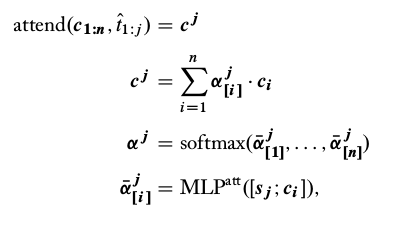
\includegraphics[scale=0.35]{pics/atten_formula.png}
\end{figure}

\item El codificador, el decodificador y el mecanismo de atención se entrenan conjuntamente para interactuar bien entre sí.
\end{itemize}

\begin{figure}[h]
  \centering
  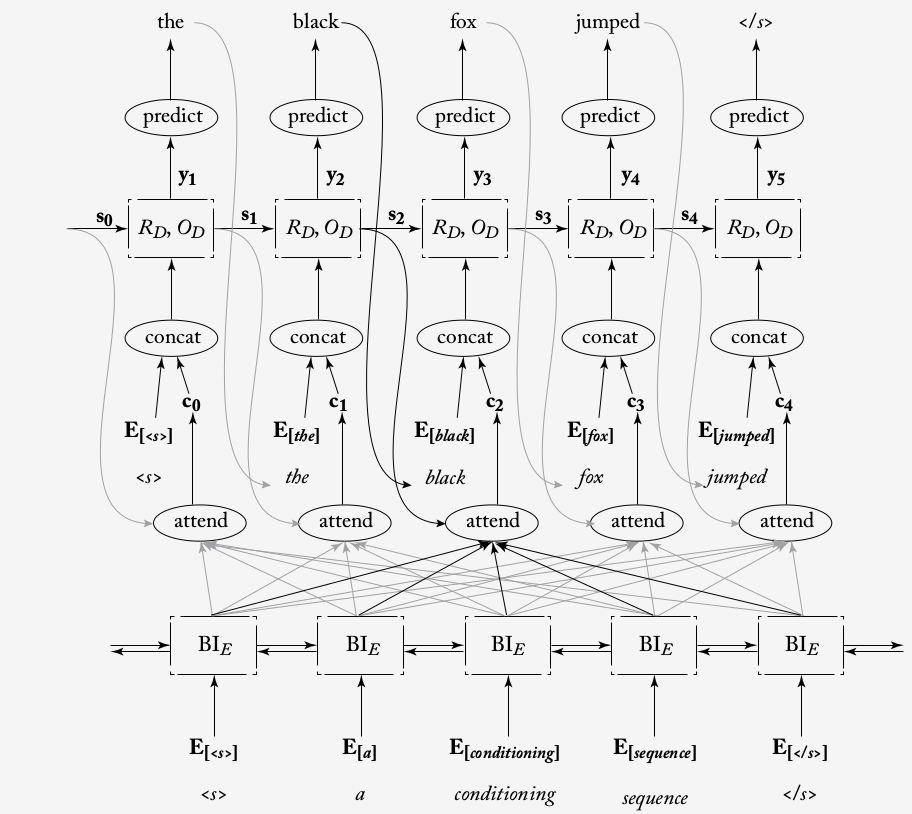
\includegraphics[scale=0.35]{pics/encdecattention.png}
  \caption{Arquitectura de un modelo codificador-decodificador con atención.}
\end{figure}

La generación de toda la secuencia a secuencia con atención se define como:

\begin{figure}[h]
  \centering
  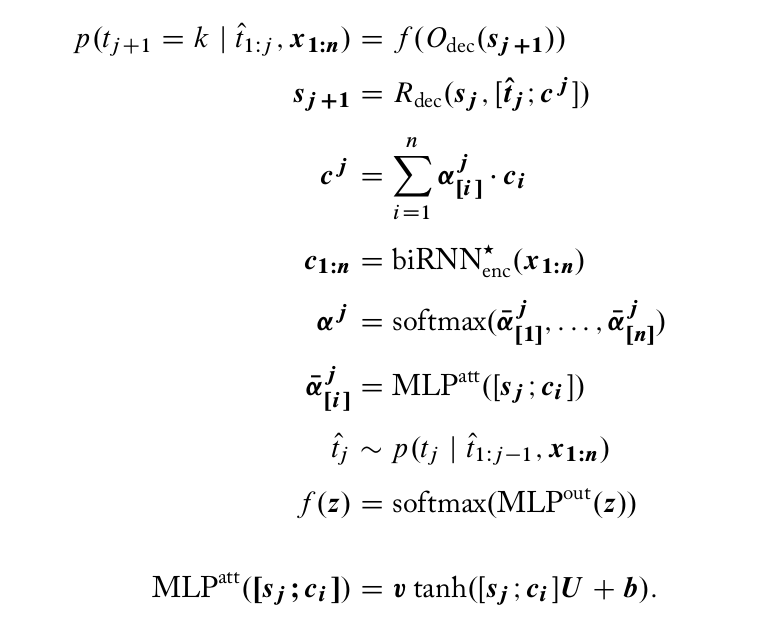
\includegraphics[scale=0.3]{pics/attentionformula.png}
\end{figure}

\begin{itemize}
\item ¿Por qué usar el codificador biRNN para traducir la secuencia de condicionamiento $\vec{x}_{1:n}$ en los vectores de contexto $\vec{c}_{1:n}$?
\item ¿Por qué no simplemente centrarse directamente en las entradas (incrustaciones de palabras) $MLP^{att}([\vec{s}_j;\vec{x}_i])$?
\item Podríamos hacerlo, pero obtenemos beneficios importantes del proceso de codificación.
\item En primer lugar, los vectores biRNN $\vec{c}_i$ representan los elementos $\vec{x}_i$ en su contexto oracional.
\item Contexto oracional: una ventana enfocada alrededor del elemento de entrada $\vec{x}_i$ y no el elemento en sí.
\item En segundo lugar, al tener un componente de codificación entrenable que se entrena conjuntamente con el decodificador, el codificador y el decodificador evolucionan juntos.
\item Por lo tanto, la red puede aprender a codificar propiedades relevantes de la entrada que son útiles para la decodificación y que pueden no estar presentes en la secuencia fuente $\vec{x}_{1:n}$ directamente.
\end{itemize}



\section{Atención y alineaciones de palabras}
En el contexto de la traducción automática, se puede pensar que $MLP^{att}$ calcula una alineación suave entre el estado actual del decodificador $\vec{s}_j$ (capturando las palabras extranjeras recién producidas) y cada uno de los componentes de la oración fuente $\vec{c}_i$.

\begin{figure}[h]
  \centering
  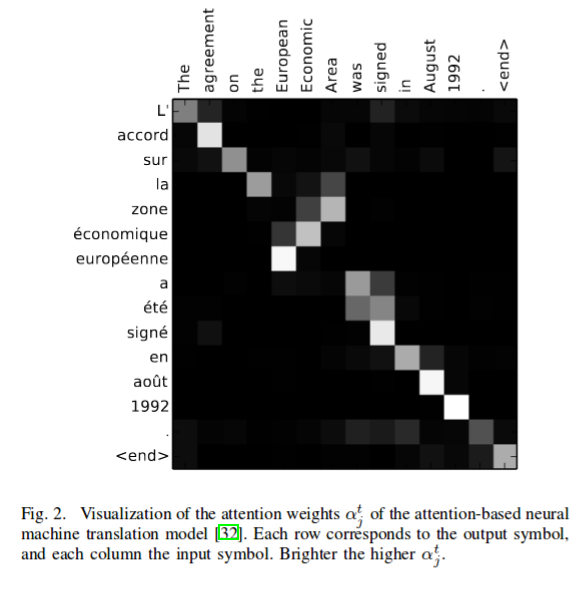
\includegraphics[scale=0.28]{pics/attention-alignment.png}
  \caption{Fuente: \cite{cho2015describing}}
\end{figure}


\section{Otros tipos de atención}
\begin{figure}[h]
  \centering
  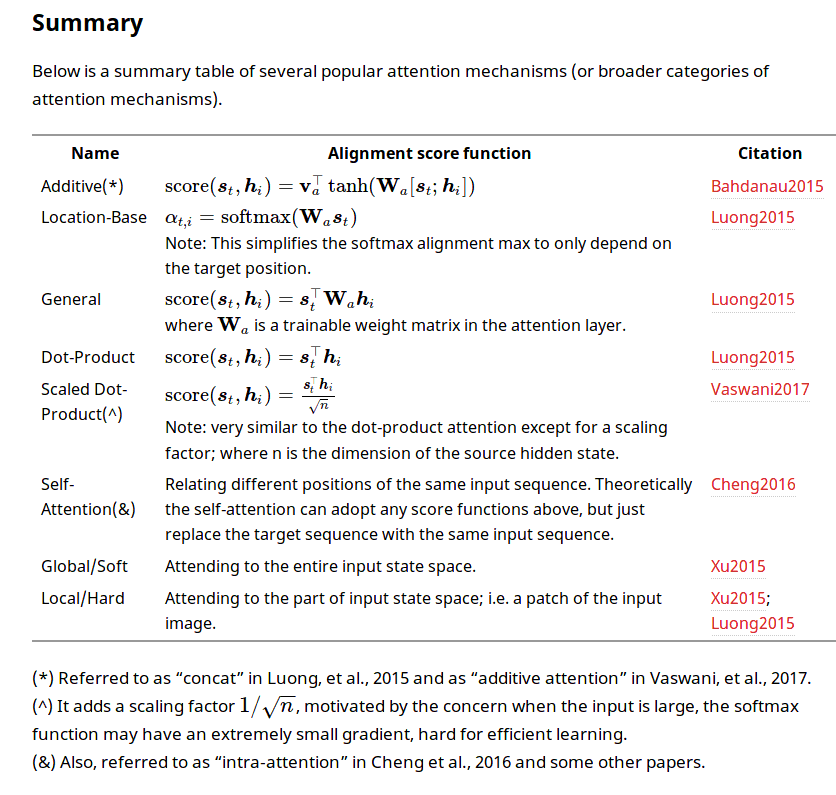
\includegraphics[scale=0.32]{pics/types_of_attention.png}
  \caption{Fuente: \url{https://lilianweng.github.io/lil-log/2018/06/24/attention-attention.html}}
\end{figure}
